\begin{figure}[hbt]
    \centering
    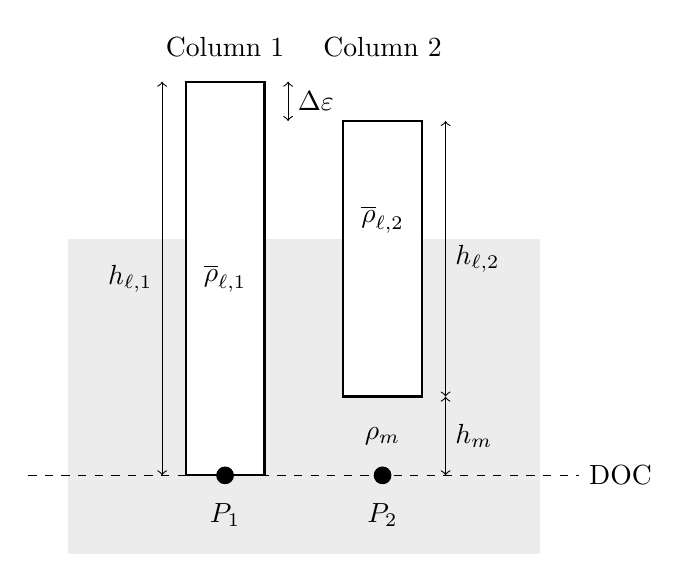
\begin{tikzpicture}[scale=1.0]

        % Asthenosphere
        \fill[gray!15] (-1.5,-1) rectangle (4.5,3);

        % Columns 1
        \draw[thick,fill=white] (0,0) rectangle (1,5);
        \node[above] at (0.5,5.2) {Column 1};
        \draw[fill=black] (0.5,0) circle (3pt);
        \node at (0.5,-0.5) {$P_1$};

        % Columns 2
        \draw[thick,fill=white] (2,1) rectangle (3,4.5);
        \node[above] at (2.5,5.2) {Column 2};
        \draw[fill=black] (2.5,0) circle (3pt);
        \node at (2.5,-0.5) {$P_2$};

        % Heights
        \draw[<->] (-0.3,0) -- (-0.3,5) node[midway,left] {$h_{\ell,1}$};
        \draw[<->] (3.3,0) -- (3.3,1) node[midway,right] {$h_m$};
        \draw[<->] (3.3,1) -- (3.3,4.5) node[midway,right] {$h_{\ell,2}$};
        \draw[<->] (1.3,4.5) -- (1.3,5) node[midway,right] {$\Delta\varepsilon$};

        % Compensation depth
        \draw[dashed] (-2,0) -- (5,0) node[right] {DOC};

        % Labels
        \node at (0.5,2.5) {$\overline{\rho}_{\ell,1}$};
        \node at (2.5,3.25) {$\overline{\rho}_{\ell,2}$};
        \node at (2.5,0.5) {$\rho_m$};

    \end{tikzpicture}
    \caption{Schematic lithospheric columns in isostatic equilibrium. Pressure is balanced at a common depth (DOC), while surface elevations differ due to variations in integrated buoyancy of each column.}
    \label{fig:columns2}
\end{figure}